\section{Social media}
\begin{frame}{Social media}{}
	\begin{itemize}
		\item Hvorfor kan steganografi brugbart?
		\item Det etiske spørgsmål
	\end{itemize}
	\begin{figure}[!H]
			\centering
			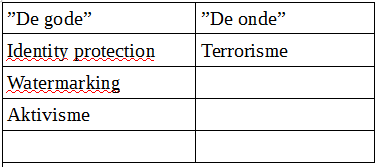
\includegraphics[width=.55\textwidth]{./Tessa/tabel.png}
	\end{figure}
\end{frame}
%%%%%%

\section{Problemformulering}
\begin{frame}{Problemformulering}{}
	\begin{itemize}
		\item How do we modify the graph-theoretic approach for steganography described in section 2.9 to work with JPEG images where the data is hidden in the DCT coefficients without significant visual changes, and how do we implement this in an object-oriented programming language?
	\end{itemize}
\end{frame}
